\documentclass[8pt]{article}
\usepackage{xcolor}
\usepackage{hyperref}
\hypersetup{urlcolor=blue}
\usepackage{times}
\usepackage{pstricks}
\usepackage{listings}
\usepackage{enumerate}
\usepackage{pst-all}
\usepackage{color}
\usepackage{pstcol,pst-node,pst-coil}
\usepackage[dvips]{graphics}
\usepackage{amsfonts,amsmath,amsthm,amssymb,euscript,amscd}
\usepackage[english]{babel}
\usepackage[autostyle]{csquotes}
\usepackage[all,cmtip]{xy}
\usepackage{float}
\usepackage{pdfpages}
\pagestyle{headings}
\setlength{\parindent}{3ex}
\setlength{\parskip}{1.5ex plus0.5ex minus 0.5ex}
\setlength{\textwidth}{14cm}
\setlength{\oddsidemargin}{1cm}
\setlength{\evensidemargin}{1cm}
\setlength{\textheight}{20.5cm}
\newcommand{\newln}{\\&\quad\quad{}}
\newcommand{\parenthnewln}{\right.\\&\left.\quad\quad{}}
\newcommand{\sub}{\subset} 
\newcommand{\T}{\mathcal{T}}
\newcommand{\R}{\mathbb{R}} 
\newcommand{\U}{\mathcal{U}}
\newcommand{\B}{\mathcal{B}}
\newcommand{\C}{\mathcal{C}}
\newcommand{\8}{\bar}
\newcommand{\maps}{\mapsto}
\newcommand{\norm}[1]{\left\lVert#1\right\rVert}
\newcommand{\e}{\epsilon}
\newcommand{\del}{\delta}
\newcommand{\f}{\frac}
\newcommand{\ol}{\overline}
\newcommand{\la}{\langle}
\newcommand{\ra}{\rangle}
\newcommand{\Par}{\partial}
\renewcommand{\qedsymbol}{\rule{0.7em}{0.7em}}
\newtheorem{theorem}{Theorem}[section]
\newtheorem{lemma}[theorem]{Lemma}
\newtheorem{proposition}[theorem]{Proposition}
\newtheorem{corollary}[theorem]{Corollary}


\begin{document} 
\title{The Science of Decisions} 
\author{\textit{Kris Anaya}}
\date{\today} 
\maketitle

\begin{abstract} 
\textit{In a Stroop task, participants are presented with a list of words, with each word displayed in a color of ink. The participant's task is to say out loud the color of the ink in which the word is printed. The task has two conditions: a congruent words condition, and an incongruent words condition. In each case, we measure the time $\textbf{t}$, it takes to name the ink colors in equally-sized lists. Each participant will go through and record a time from each condition.} 
\section{Introduction}
In this task, we are asked to measure the time it takes to name the ink colors in equally-sized lists. In the \textit{congruent} words, the words that are displayed are color words whose names match the colors in which they are printed. In the \textit{incongruent} words conditions, the words displayed are color words whose names do no match the colors in which they are printed. Meaning, what is the probability it takes our independent variable $t$ to name the colors in the \textit{congruent} and \textit{incongruent} words within these two independent samples which are dependent on $t$: 
\begin{equation} 
P(X = congruent \mid Y = incongruent) 
\end{equation} 
Within this project we test that there is no significant change in speed between the  \textit{congruent} and \textit{incongruent} samples. However, this will be tested against alternative changes between our \textit{congruent} and \textit{incongruent} samples given our independent variable $t$ at $\alpha = 0.05$: 

\begin{equation}
\begin{split}
H_{0}: \mu_{c}-\mu_{I} = 0 \\
H_{A}: \mu_{c}-\mu_{I} \not= 0 
\end{split}
\end{equation}
We will perform these task by using a Pythonic language module which we have created. This module is aptly named \textit{statistics.py}. 
The resources for our code may be found within our GitHub page \textit{http://github.com/krismanaya} under \textit{UdactiyDataScience}. Within our methods, we may conclude that a Type I error is very unlikely. Therefore, the test procedure will be based on a rejection $H_{0}$ at an $\alpha$ level of $0.05$. In conclusion, we will show there is a significant difference between naming \textit{congruent} and \textit{incongruent} colors by relying on our independent variable $t$. 
\newpage
\section{Methods}
\subsection{sample} 
The sample population of interest is taken from the Stroop dataset provide by the Udacity Class. This data set may be viewed on Udacity's Google drive \href{https://drive.google.com/file/d/0B9Yf01UaIbUgQXpYb2NhZ29yX1U/view}{website}. The sample population that is provided consists of a list of patients who were tested twice, one saying the words with applying the \textit{congruent} method and then tested again saying the word with the \text{incongruent} method. Both samples were done under $t$ constraint. 
\subsection{design} 
A repeated measures longitude two-test randomized experimental design was provided for this study. We wish to analyze the effect size of the given treatments. The given variables  and measures will be the mean, size, standard-error, t-statistics, confidence interval; degrees of freedom, t-critical and Bessel's approximation.These measures and variables will be denoted as:
\newline
\newline
\newline

\fbox{\parbox{\textwidth}{\textit{Stroop variables:}
\begin{enumerate}
\item $\bar{X}_{c} :=$ congruent mean 
\item $\bar{X}_{I} :=$ incongruent mean 
\item $N_{c,i} := $ size of  list
\item $\alpha :=$ alpha level 
\item $t_{c} :=$ t-critical interval 
\item $t_{stat} :=$ t-statistic 
\item $df :=$ degrees of freedom 
\item $SE :=$ standard error 
\item $\sigma_{c,i} :=$ standard deviation (Bessel) 
\item $CL :=$ confidence level 
\end{enumerate}}}
\newline
\newline
Within this design we test that there is no significant change in speed between the \textit{congruent} and \textit{incongruent} samples. However, this study will be tested against alternative changes between our $H_{0}$ given our independent variable $t$ at $\alpha = 0.05$: 
\begin{equation}
\begin{split}
H_{0}: \mu_{c}-\mu_{I} = 0 \\
H_{A}: \mu_{c}-\mu_{I} \not= 0 
\end{split}
\end{equation}
\newpage
\section{Results} 
\subsection{variability} 
Within the results section we round all data points two decimals places. We begin by locating the variables, we used our Pythonic module \textit{statistics.py} to create a two-list aptly named \text{congruent} and \textit{incongruent}. Secondly, we calculated the mean $\bar{X}_{c,i}$ and $\sigma_{c,i}$ with help of our functions: 
\begin{table}[htbp]\centering \caption{Stroop statistics \label{sumstat}}
\begin{tabular}{l c c  }\hline\hline
\multicolumn{1}{c}{\textbf{Variable}} & $\bar{X}$ & $\sigma$ \\ \hline
Congruent & 14.05 & 3.56  \\
Incongruent & 22.02 & 4.80  \\
\multicolumn{1}{c}{n} & \multicolumn{2}{c}{24}\\ \hline
\end{tabular}
\end{table}
\small{\begin{verbatim}
congruent = make_a_list() 
incongruent = make_a_list() 
x_c = mean(congruent) 
>>> 14.05
x_i = mean(incongruent)
>>> 22.02 
sigma_c = bessels_correction(congruent) 
>>> 3.56
sigma_i = bessels_correction(incongruent) 
>>> 4.80 
\end{verbatim}}
\noindent The reader may have observed that within the mean and standard deviation, the length and average $t$ is much smaller for our congruent list of data points. This may suggest to us that the first test has an overall faster time of saying words. 
\subsection{central tendencies} 
Within our central tendencies we wish to calculate the standard error, t-statistic, degrees of freedom and t-critical at $\alpha = 0.05$: 
\begin{table}[htbp]\centering \caption{Stroop statistics \label{sumstat}}
\begin{tabular}{l c c  }\hline\hline
\multicolumn{1}{c}{\textbf{Central Tendencies}} \\ \hline
$SE$ & 1.22\\
$df$  & 46 \\
$t_{stat}$ & -6.53  \\ 
$t_{c}$ &  2.009 \\ 
$\alpha$ & 0.05 \\
\multicolumn{1}{c}{CL} & \multicolumn{2}{c}{.95}\\ \hline
\end{tabular}
\end{table}
\begin{verbatim}
SE = independent_standard_error(congruent,incongruent,len(congruent),len(incongruent)) 
>>> 1.22 
df = degrees_of_freedom_indy(congruent,incongruent) 
>>>  ((24, 24), 46)
t_stat = t_stat_indy(x_c,x_i,0,0,sigma_c,sigma_i,24,24)
>>> -6.53 
# t_c = use chart* 
\end{verbatim}
Here we visualize a t-distribution at $\alpha$ level denoted above and at $0.95$ confidence interval. As we can see our $t_{stat}$ variable is well below the critical value. This suggests that it is possible there is some significant changes between the \textit{congruent} and \textit{incongruent}. Because of this we shall reject $H_{0}$ and conclude that there exist a probability $P < \alpha$.
\begin{figure}
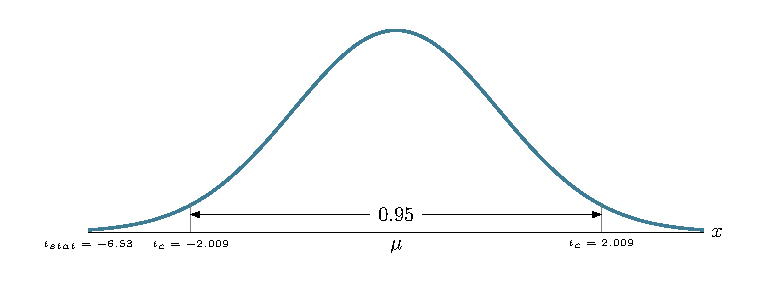
\includegraphics[page=1,scale=0.8]{t-distro.pdf}}
\end{figure}

\section{Discussion}
The effects responsible for a rejection of $H_{0}$ could be due to the patient's eyes becoming comfortable with words and colors that when they are ready to observe the \textit{incongruent} test their eyes have still not settled. One test you could do is switch the test and perform a Stroop task of \textit{incongruent} then \textit{congruent} and see if the samples differ. Another similar approach for the test would make the patient perform the task multiple times to see if there is some level of improvement after practicing the \textit{incongruent} tests. Finally, a last possibility could be age and eyesight. Do these patients are different in age are they similar? What are the patients eyesight, is it normal or do some patients struggle with color? We do not have more information within the data set. The only information given to us is the independent variable $t$. 
\end{document} 